\documentclass[11pt]{article}

\usepackage[utf8]{inputenc}
\usepackage[english]{babel}
\usepackage{graphicx}
\usepackage[margin=1in]{geometry}
\usepackage[parfill]{parskip}
\usepackage{listings}
\usepackage{color}
\usepackage{float}


\title{LPHY1300 Personal project report :\\ Simulation of a particle detector}
\author{\textsc{Schils} Arnaud\\ \textsc{Lardinois} Simon}
\date{2015-2016}

\begin{document}

	\lstset{language=C++,
	                basicstyle=\ttfamily,
	                keywordstyle=\color{blue}\ttfamily,
	                stringstyle=\color{red}\ttfamily,
	                commentstyle=\color{green}\ttfamily,
	                morecomment=[l][\color{magenta}]{\#}
	}
\maketitle
\newpage
\renewcommand{\contentsname}{Table of contents}
\tableofcontents




\newpage
\section*{Introduction}

Nowadays, the huge amount of computing power offered by modern computer systems allows
to solve complex scientific problems numerically. The art of solving physics problems using
computers is referred as \textit{computational physics}. This modern field
is multidisciplinary: it brings together applied mathematics,
computer science and physics. If offers a third way to do physics
that supplements theory and experiment.

In this thesis, these numerical techniques are applied to the field of particle
detectors physics. In order to design the best detectors,
physicists have to know the measured signal resulting from the passage of a particle
in the detector. Unfortunately, due to the complex geometries of these detectors
and the various physical phenomena to handle, this signal is not easy
to compute analytically.

It is why, in the context of this thesis, a software  to compute the current measured
by a particle detector due to the passage of a particle has been developed.
This software has then been used to study silicon and gas particle detectors.

	% In the context of our lesson LPHY1300 personal project, we
	% had to simulate a particle detector using the finite elements method. We
	% thus develop our program "pdetect" which simulates the electric potential
	% and electric field inside a pixel detector. It also computes the electric
	% current induce by an incident particle with a given trajectory.

	\subsection*{Overview of the contributions}

	The primary contribution of this thesis is the development of a C++ numerical software performing the
	following tasks.

	Firstly, it computes the potential and the electric field
	at each point of a particle detector solving the Laplace equation for non-trivial
	two-dimensions geometries. Three types of 2D detector geometries are supported.
	The Laplace equation is solved using the \textit{finite element method} with an adaptive
	grid refinement strategy. The software supports multithreading and therefore
	uses all available CPUs to quickly solve this equation.

	Secondly, the software computes the current resulting from the passage of a particle
	in the detector using the \textit{Shockley–Ramo theorem} and the solution of the
	computed electric field. Every possible particle trajectories in the detector
	are suppoted. Effects such as the \textit{mobility} difference between holes and
	electrons, the \textit{saturation} phenomena and the \textit{Townsend Avalanche}
	are handled.

	This software has been developed following the object-oriented
	programming paradigm and with the \textit{model-view-controller}
	software engineering pattern in mind. Thanks to the quality of the software
	architecture further extensions such as 3D geometries, additional physical effects or
	detector types and the support of distributed computations on clusters are possible
	without the burden of reimplementing an entire new software.

	The secondary contribution of this thesis is the use of this software to study
	the gas and silicon detectors. Finally, the results provided by the
	software have been compared with the results of \textit{Weightfield}~\cite{Cenna2015}, a
	software performing similar computations.

	%To perform this task, the software places charges
	%resulting from the ionization of the molecules inside the detector. Then, these
	%charges drift following the applied potential at the anode and cathode of the detector

	\subsection*{Organization of the thesis}

	TODO

	% In this paper we will first introduce briefly what the finite elements
	% method is, and then a library we used in our program, "deal.II".
	% After what we will explain properly our program, the way it works, and
	% also comparing our results with the results of "weightfield", another
	% simulator of a particle detector, already use in many experiences.
	% To finish this paper we will talk about two specific cases of detector,
	% a silicon detector, and a helium detector.


\section{Background and related work}

This section is composed of three parts. Firstly,
 the finite element method is briefly explained. Then \textit{deal.ii},
 a C++ library implementing the finite element method is introduced. Finally,
 \textit{Weightfield}, another software performing particle detector simulation,
 is presented.

	\subsection{Finite element method}

		The finite element method is a numerical technique for
		finding approximate solutions to boundary value problems for partial
		differential equations. The finite element method subdivides a large
		problem into smaller, simpler, parts, called finite elements. The
		simple equations that model these finite elements are then assembled
		into a larger system of equations that models the entire problem. It
		then uses variational methods from the calculus of variations to
		approximate a solution by minimizing an associated error function.

	\subsection{Deal.II library}

	In order to avoid to reinvent the wheel, it was decided to use the deal.ii library
	to solve the Laplace equation~\cite{Bangerth:2007:DGO:1268776.1268779}. This decision allows to rely on the optimized
	and robust code of deal.ii and to benefit from the cutting edge numerical methods this library provides.

	deal.II is a C++ library allowing to solve partial differential equations
	using the finite element method. It is a very powerful but low-level library.
	It offers several features such as adaptive meshes, grid handling
and refinement, handling of degrees of freedom, input of meshes and output of results in
graphics formats. Furthermore, deal.ii allows to easily write code that works
for any dimensions because code using deal.ii is written independently of the space
dimension. Thanks to this design choice, the code of our software is quite easily
extensible to 3D.

Finally, deal.ii supports multithreading as well as \textit{MPI~\footnote{Message
Passing Interface. MPI is used to develop distributed softwares running on top of
clusters of computers.}}. Therefore,
deal.ii is able to hardness the power of multithreaded CPUs as well as
clusters composed of hundreds of computers. Consequently,
the software developed in this thesis is multithreaded and could be extended to
exploit the resources offered by clusters.


	\subsection{Weightfield}

Weightfield is a program to study the performance of silicon and diamond
detectors~\cite{Cenna2015}. It simulates the energy released by particles in the detector
and uses the Ramo's theorem to compute the signal current.

Among others, Weightfield allows to play with the following parameters:
sensor geometry, internal gain, doping of silicon sensor and its operating
conditions, the application of a magnetic field, the ambient temperature and
thermal diffusion.

Weightfield has been used in this thesis to compare and valid the results
obtained with our own software.

\section{Introduction to the physics of particle detectors}

In this section, the concepts of particle detectors physics used in this project
are introduced.

A particle detector is composed of a cathode, an anode and an active media
between them (gas,...). A potential difference is applied between the cathode
and the anode~\cite{lphy2236}.

When a particle pass through the active media, the radiation ionizes the media
molecules along the particle trajectory.
Because of the applied potential difference,
produced ion-electron pairs drift inside the detector until they reach the anode
(for the ions) or the cathode (for the electrons). These ions and electrons
are moving charges and therefore produce a current.

The number of ion-pairs per length $n_{eff}$ produced in the media by the
particle passage is given by the following formula:

\[n_{eff} = \frac{dE/dx}{w} \]

where $dE/dx$ is the energy deposited by the particle in the media by
unit of length, and $w$ is the average energy to produce one ion-pair.

The charges drift in the detector media with a velocity function of the electric
field and the mobility~\cite{spieler2005semiconductor}:

\[\vec{v} = \mu \vec{E}\]

where $\mu$ is the \textit{mobility}. Electrons and holes (or ions) have different
mobilities. For example, in Silicon, mobilities are 1350 and 450 $cm^2V^{-1}s^{-1}$,
respectively. In gas, the mobility difference between electrons and holes is
much larger, electrons are typically a thousand times faster ($\mu =$ 100 $cm^2V^{-1}s^{-1}$
for electrons and $\mu =$ 0.1 $cm^2V^{-1}s^{-1}$ for holes). Notice that the mobility
is not a constant in general.

Due to saturation, the mobility decreases when fields of 104 $V cm^{-1}$ and higher are applied in
the detector following the relation:

\[\mu_s = \mu \left (1 + \left (\frac{\mu |E_y|}{v_{sat}} \right )^{\beta} \right )^{-\frac{1}{\beta}}\]

where $\beta$ is a constant, $\mu$ the mobility when not considering saturation,
$E_y$ the component of the electric field along the axis orthogonal to the anode and cathode
and $v_{sat}$ the saturation velocity. The saturation velocity depends on the
media and the temperature.

Once the velocity is known, the current generated by moving ion-electron
pairs can be computed. The Shockley–Ramo theorem states that the instantaneous current generated
by one moving charge $q$ at velocity $\vec{v}$ is:

\[i = -q \vec{v} \cdot \vec{E}_w\]

where $q$ is the signed charge and $\vec{E}_w$ is the \textit{weighting field}. The weighting field is the electric field
obtained when applying a potential of $1V$ to the measurement electrode and setting
the potential of the other electrodes to $0V$.

The instantaneous current measured
by the detector is the sum of the currents generated by the holes and electrons:

\[i_{tot} = \sum_{holes} i_h + \sum_{electrons} i_e\]

An additional effect to take into account  when dealing with gas detectors is
\textit{charge multiplication}~\cite{lphy2236}. This effect
multiplies the primary ionization charges by an avalanche phenomena.
The \textit{Townsend avalanche} is implemented in our software. It happens
when the electric field is higher than $10^6Vm^{-1}$. The electrons collide
with the molecules of the media and, if their kinetic energy is sufficient,
extract additional electrons from this molecules.

The Townsend avalanche multiplies the local number of electrons (and therefore the local electric
charge) if the electric field is high enough and if the electrons are close
to the cathode. When these conditions are fulfilled, during a time interval
$\Delta t$ the initial electric charge $q_0$ is multiplied
according to the formula:

\[q = q_0 e^{\alpha \Delta x}\]

where $\Delta x$ is the distance covered by the electron and $\alpha$ the
\textit{first Townsend coefficient}. This coefficient is computed as follows:

\[\alpha = ap \ e^{-bp/E}\]

where $a, b$ are constants depending on the gas media, $p$ the pressure in
the detector (the atmospheric pressure is commonly used) and $E$ the norm
of the electric field at the charges position.

\section{Software features}

This section first presents the features of the software. Firstly,
the implemented detector geometries are presented. Secondly, some details
about the resolution of the Laplace equation are provided. Thirdly, the
computation of the current measured by the detector is described.

The software handles three types of 2D geometries:

\begin{enumerate}
\item \texttt{Middle circular holes rectangle}: this geometry is a rectangle with circular
holes vertically centered and uniformly distributed along the horizontal axis (see
Figure~\ref{fig:mid_circle_geometry}). The configurable values of the geometry
are the rectangle width,
the hole radius, the inter holes centers distance and the number of holes.
The potential is set to $0V$ at the top and bottom boundaries. Left and right
boundaries have free boundary conditions.

\begin{figure}[H]
  \center
  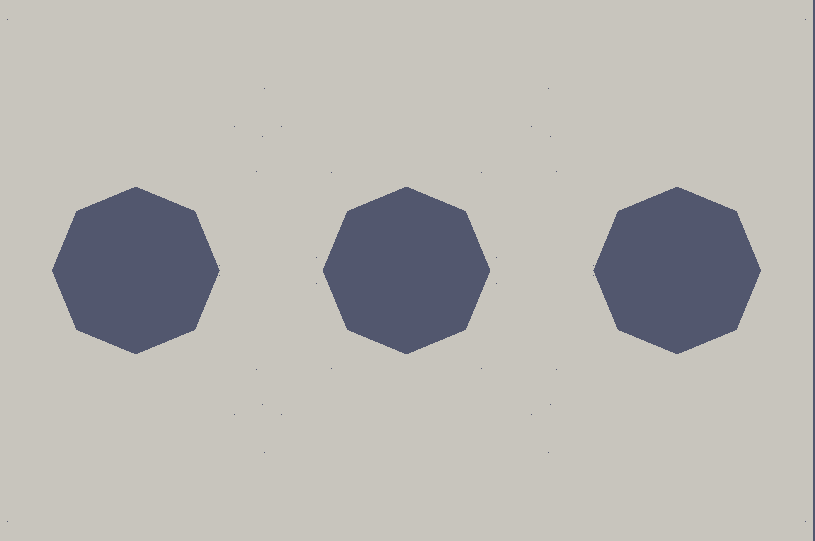
\includegraphics[scale=0.2]{images/mid_circle_geometry.png}
  \label{fig:mid_circle_geometry}
  \caption{Middle circular holes rectangle geometry.}
\end{figure}


\item \texttt{Middle rectangular holes rectangle}: this geometry is a rectangle with rectangular
holes vertically centered and uniformly distributed along the horizontal axis
(see Figure~\ref{fig:mid_rect_geometry}).
The configurable values of the geometry are the rectangle width, the number of
holes, the inter holes distance, the hole width and the hole length.
The potential is set to $0V$ at the top and bottom boundaries. Left and right
boundaries have free boundary conditions.

\begin{figure}[H]
  \center
  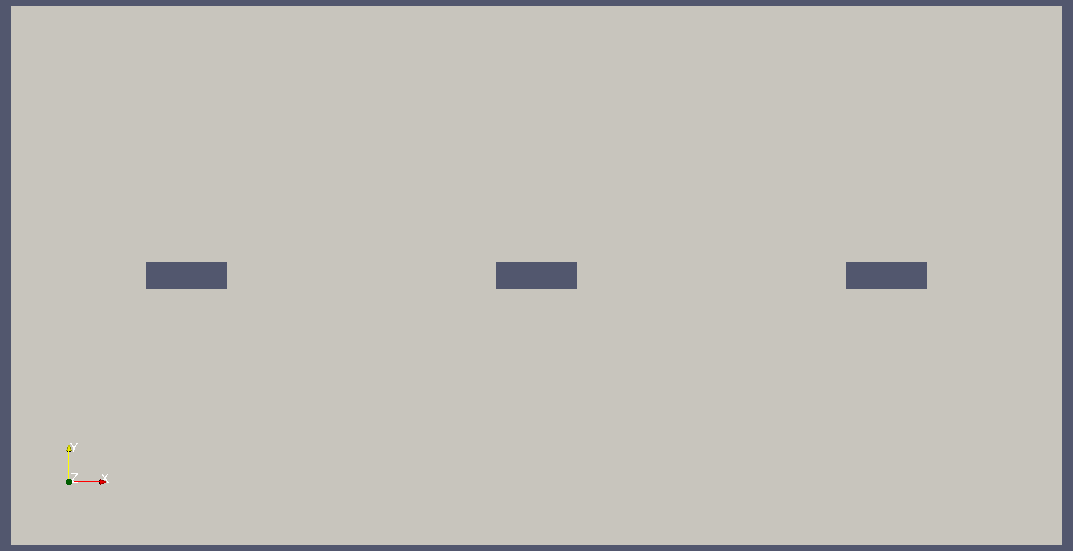
\includegraphics[scale=0.2]{images/mid_rect_geometry.png}
  \label{fig:mid_rect_geometry}
  \caption{Middle rectangular holes rectangle geometry.}
\end{figure}


\item \texttt{Serrated rectangle}: this geometry is a rectangle with periodic
holes inserted near the top boundary, along the horizontal axis
(see Figure~\ref{fig:serrated_rect_geometry}).
The configurable values of the geometry are the rectangle width, the number
of holes, the hole length (i.e. the length of the side parallel to the top
rectangle boundary), the hole width and the inter holes space.
These holes are the potential sources, the boundary value at their borders is therefore
the strip potential. The holes inter-spaces have free boundary conditions.
The right and left boundaries of the rectangle have free boundary conditions as well.
Finally, the value at the bottom boundary is 0V.

\begin{figure}[H]
  \center
  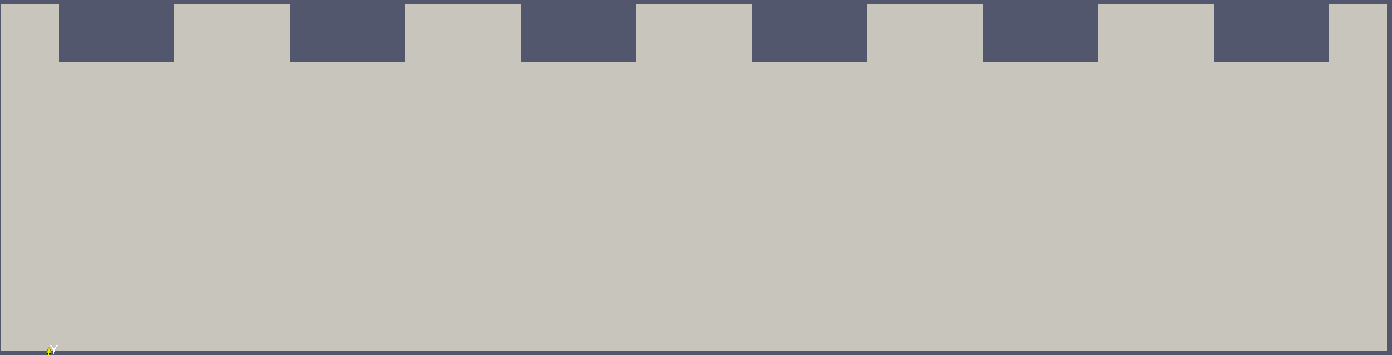
\includegraphics[scale=0.2]{images/serrated_rect_geometry.png}
  \label{fig:serrated_rect_geometry}
  \caption{Serrated rectangle geometry.}
\end{figure}
\end{enumerate}


For each one of these geometries, a coarse grid (or mesh) is generated using
functions of the \texttt{deal.ii} library.

Once the grid is generated, the Laplace equation is solved for the considered
geometry. This is achieved using all available CPU cores and in several iterations.
At the first one, the
grid is coarse and the error on the computed results is high. Then, the grid is
refined only at cells with the largest errors and the Laplace equation is
solved on this denser grid. This process continues until
the error is smaller than a relative error provided by the user at each cell of
the grid. This is adaptive grid refinement. It allows to achieve good precision
everywhere in the grid without losing time refining cells where the error is already small
enough.

The result of the Laplace equation is of course the potential at each point of
the grid. The gradient of the potential is available as well at
the end of this process. A graphical representation of both the potential and
its gradient can be written in a \texttt{vtk} file.
These files can be read by the \texttt{Paraview} software.

The same process is performed with different boundary conditions in order
to compute the weighting potential and the weighting electric field.

For each cell of the grid, the values of the potential, the error of the
potential and the electric field are stored in a \texttt{rtree} data structure.
In the algorithm computing the current measured by the detector, these three
values have to be retrieved from the coordinates of a point. In order to retrieve the proper
values, it is required to know to which cell the point belong. Since the grid
is not uniformly refined, it is not easy to efficiently find this cell.
Iterating through each cell of the grid is far too slow especially when 3D
geometries will be introduced in the software. The algorithm finding the cell
to which a point belong would have a $\mathcal{O}(n)$ time complexity, where $n$
is the number of cells in the grid. The \texttt{rtree} data structure
performs this search with a $\mathcal{O}(log(n))$ time complexity.

The software then uses these results to compute the current measured by the
detector. The user has to specify the particle trajectory. Any trajectory is
supported. The computation of the current is composed of the following steps.

Firstly, the ion-pairs generated by the particle pass are placed at their initial
positions inside the detector. At this end, the intersections points between the
detector boundaries and the particle
trajectory are computed. Notice that a particle may enter and leave the detector
several times (the potential sources, or strips, are not considered as being
part of the detector). It happens for example if the particle trajectory is
horizontal near the top boundary of a serrated rectangle geometry.
The segments being part of both the particle trajectory and the detector
geometry are retrieved. The total
distance covered by the particle inside the detector is then computed as
the sum of the length of these segments. From this, the total number of ions-pair
created by the particle pass is computed
as the product of the covered distance with the number of ions-pair created by unit
of length. The number of ions-pair created by unit
of length is considered as a constant and is different from one
media to another. Depending on the precision level specified by the user, the
total number of ions-pair
is uniformly spread along the path covered by the particle inside the
detector. When the precision is higher, the total number of pairs is spread
among more points. On the opposite, if the precision level is set to 0,
the whole ion-pairs are placed at the same point.

\section{Software architecture}

This software is developed in C++ with the object-oriented programming paradigm.
This section presents how the software is divided in several modules. Each module
is composed of different classes.

The program main function calls functions from the \texttt{test} folder. These functions
assemble the different objects to perform the required computation. In the
final version of the program, functions of the test folder should be replaced
by a graphic user interface: a \texttt{view} and a \texttt{controller} following
the model-view-controller software engineering pattern. In this pattern code
related to core of the program functionality (the \texttt{model}: mathematical computations, file access,...)
is separated from the code related to the user interface (the \texttt{view}).
The \texttt{view} and the
\texttt{model} are connected by the \texttt{controller} module.

The main advantage of this design pattern is to be able to change the user interface without
performing any modification to the code of the \texttt{model} module. Furthermore,
mixing model and graphic interface related code should be avoided because it leads to
less readable and not modular code.

The graphic user interface would allow the user the specify
parameters of the simulation at runtime rather than hardcoding parameters
directly in the functions of the \texttt{test} folder.
The development of the \texttt{controller} and \texttt{view} modules
is left for future work. The reminder of this section presents the most important classes
included in the \texttt{model} module.

The \texttt{MyGeometryInfo} abstract class contains (and provides) informations
related to the
geometry of the detector as well as methods to compute the intersections of a
line with the boundaries of the geometry and to check if a point is inside
the geometry. This abstract class has three implementations:





The \texttt{Detector2D} class is an abstract class that models a detector
represented by a two-dimensional geometry (a section of a detector). Classes
implementing this abstract class must implement the following methods:
% \begin{itemize}
% 	\item \lstinline{void comp_potential()}: this method computes the potential
% 	at each point of the detector.
% 	\item \lstinline{void comp_weight_potential()}: this method computes the
% 	weighting potential	at each point of the detector.
% 	\item \lstinline{MyGeometryInfo* get_geometry_info()}
%
% 	\item \lstinline{void get_solution(Solution<2> &sol)}
%
% 	\item \lstinline{void get_solution_weight(Solution<2> &sol)}
%
% 	\item \lstinline{Hole get_hole()}
%
% 	\item \lstinline{Electron get_electron()}
%
% 	\item \lstinline{double get_hole_pairs_nbr_per_lgth()}
%
% 	\item \lstinline{double get_strip_potential()}
%
% 	\item \lstinline{double get_first_townsend_coefficient(Point<2> &pos, PhysicalValues<2> &values_at_pos)}
%
% 	\item \lstinline{unsigned electric_charge_multiplicator(}
%
% 	\lstinline{Point<2> &pos,Charge *charge,PhysicalValues<2> &values_at_pos,double &displacement)}
%
% 	\item \lstinline{virtual std::string params_to_string()}
%
% 	\item \lstinline{draw_vtk_graph_*}: this set of methods output some \texttt{vtk}
% 	files. These files contain a graphic representation of the potential and
% 	electric field. These files can be read by the \texttt{Paraview} software.
%
%
% \end{itemize}


\subsection{Flow of Execution}

This section presents the actions performed by the program in chronological
order.



%Functions from the \texttt{test} folder first instatiates an object of

\section{Results for silicon and gas detectors}

\section{Future work}

\section{Conclusion}

\newpage

\bibliographystyle{plain}
\bibliography{report.bib}

\end{document}
